\documentclass[../../topologia_algebraica]{subfiles}
\begin{document}
\section{Lazos}
\begin{defin}
  Sea $X$ un espacio topol\'ogico y $x_0\in X$. Un \emph{espacio basado} es la pareja
  $(X,x_0)$ y un morfismo $f:(X,x_0)\ra(Y,y_0)$ entre espacios basados es una funci\'on
  continua $f:X\ra Y$ tal que $f(x_0)=y_0$.
\end{defin}

Observemos que la clase de espacios basados junto con los morfismos de espacios basados
forman una categor\'ia que denotamos por $\mathbf{Top}_*$ (aqu\'i la notaci\'on viene de
$\mathbf{Top}$, la categor\'ia de espacios topol\'ogicos). Esto se sigue inmediatamente
de que la composici\'on de funciones continuas es continua.

\begin{defin}
  Sea $(X,x_0)$ un espacio basado. Un \emph{lazo} en $(X,x_0)$ es una funci\'on continua
  $\alpha:[0,1]\ra X$ tal que $\alpha(0)=x_0=\alpha(1)$, es decir, una curva cerrada. Al
  conjunto de todos los lazos en $(X,x_0)$ se denota por
  \[
    \Omega(X,x_0):=\{[0,1]\morf{\alpha} X \mid \alpha\;\text{es una lazo en}\;(X,x_0)\}.
  \]
\end{defin}
\begin{ejemplo}\label{ejemplo:lazo}$\;$\\
  \begin{enumerate}
  \item La funci\'on constante $c(s)=x_0$ para toda $s\in[0,1]$ es claramente un lazo
    en $(X,x_0)$. De hecho se considera como el lazo trivial y funcionar\'a como elemento
    neutro en las construcciones que haremos m\'as adelante.
  \item El c\'irculo $\mathbb{S}^1$ se puede pensar como un lazo en $(\CC,1)$, o en $(\RR^2,(1,0))$;
    la funci\'on $\alpha(s)=e^{2\pi i s}$ es continua y cumple que $\alpha(0)=e^0=1=e^{2\pi i}=\alpha(1)$.
  \end{enumerate}
\end{ejemplo}

El espacio $\Omega(X,x_0)$, en general, es demasiado grande como para poder realmente detectar
propiedades topol\'ogicas de $X$. Entonces vamos a subdividir $\Omega(X,x_0)$ en clases de
equivalencia. Para esto queremos que dos lazos sean equivalentes si podemos ``deformar'' continua
un lazo en otro; de esta manera podremos aislar las propiedades topol\'ogicas de $X$.

La idea de ``deformar'' un lazo $\alpha_0$ al lazo $\alpha_1$ es realmente cambiar continuamente
de lazos hasta llegar a $\alpha_1$. M\'as precisamente, una deformaci\'on es una familia de lazos
$\{\alpha_t\}_{0\leq t\leq 1}$ que empiezan en $\alpha_0$, var\'ian continuamente mientras $t\ra 1$
y terminan en $\alpha_1$. Escribimos la definici\'on para hacer m\'as preciso esta idea.

\begin{defin}
  Sean $\alpha,\beta\in\Omega(X,x_0)$. Una \emph{homotop\'ia} entre $\alpha_0$ y $\alpha_1$
  es una funci\'on continua $H:[0,1]\times[0,1]\ra X$ tal que:
  \begin{itemize}
  \item Para toda $t\in[0,1]$ fija, $\alpha_{t}(s):=H(s,t)$ es un lazo en $(X,x_0)$.
  \item $H(s,0)=\alpha(s)$ y $H(s,1)=\beta(s)$.
  \end{itemize}
  Si existe una homotop\'ia entre dos lazos $\alpha$ y $\beta$, decimos que son
  \emph{homot\'opicos} y lo denotamos por $\alpha\simeq\beta$.
\end{defin}

\begin{ejemplo}\label{ejemplo:homotopia_lazos}$\;$\\
  \begin{enumerate}
  \item El lazo constante $c(s)=(1,0)$ y el lazo $\Sn^1$ (del ejemplo \ref{ejemplo:lazo}) son
    homot\'opicos en el espacio basado $(X,x_0)=(\RR^2,(1,0))$ mediante la homotop\'ia:
    \[
      H(s,t)=(t+(1-t)\cos 2\pi s,(1-t)\sin 2\pi s).
    \]
    Podemos pensar a $H$ como la restricci\'on de una funci\'on suave $\bar{H}:\RR^2\ra\RR^2$
    (con la misma regla de correspondencia) y as\'i concluimos que $H$ es continua. Observemos
    que para $t_0\in[0,1]$ fija cada $H(s,t_0)$ es un c\'irculo con centro $(t_0,0)$ y radio
    $1-t_0$.
%%%%%%%%%%%%%%%%%%%%%%%%%%%%%%%%%%%%%%%%%%%%%%%%%%%%%%%%%%%%%%%%%%%%%%%%%%%%%%%%%%%%%%%%%%%% FIGURA
\begin{figure}
  \caption{$\Sn^1$ es homot\'opico a un punto.}
  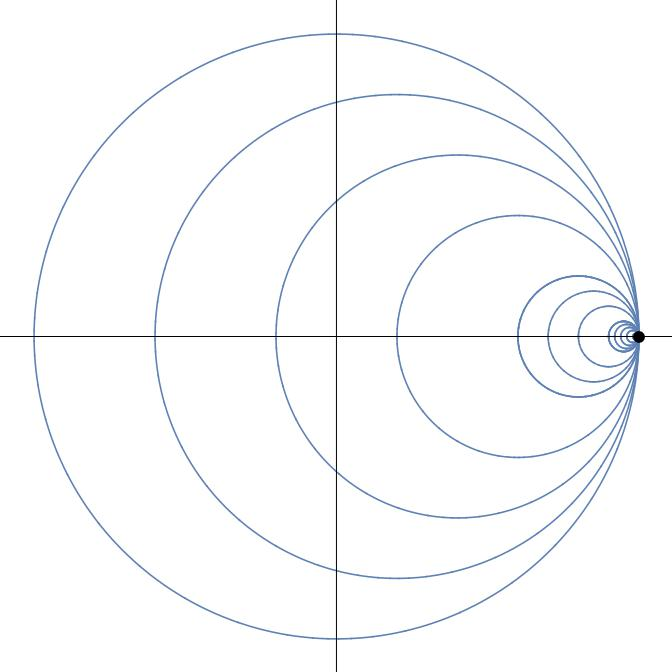
\includegraphics[scale=0.25]{circulo_homotopico_a_punto}\centering
  \label{fig:circulo_homotopico_a_punto}
\end{figure}
%%%%%%%%%%%%%%%%%%%%%%%%%%%%%%%%%%%%%%%%%%%%%%%%%%%%%%%%%%%%%%%%%%%%%%%%%%%%%%%%%%%%%%%%%%%%
    Por lo tanto es un lazo en $(\RR^2,(1,0))$ porque
    \[
      H(0,t_0)=(t_0+(1-t_0)\cos 2\pi 0,(1-t_0)\sin2\pi 0)=(1,0)=H(1,t_0)
    \]
    para toda $t_0\in[0,1]$ ($H$ es una funci\'on peri\'odica en $s$ con periodo 1), v\'ease
    la figura \ref{fig:circulo_homotopico_a_punto}.

    Por \'ultimo $H(s,0)=(\cos2\pi s,\sin 2\pi s)$ es el c\'irculo $\Sn^1$ y $H(s,1)=(1,0)=c(s)$ es
    el punto y as\'i, $H$ es una homotop\'ia entre $\Sn^1$ y el lazo constante $c(s)$. Por lo tanto
    $\Sn^1\simeq c$ en $(\RR^2,(1,0))$.

  \item Si tomamos $(X,x_0)=(\RR-\{0\},2)$, entonces el lazo $\alpha(s)=2+\sin2\pi s$ es homot\'opico al
    lazo constante $c(s)=2$, mediante la homotop\'ia $H(s,t)=2+(1-t)\sin 2\pi s$ (la prueba de este
    hecho es id\'entico al ejemplo anterior; la idea es que el factor $1-t$ hace que las osilaciones
    del lazo cada vez se hacen m\'as peque\~nas hasta que termina por no osilar y se fija en el 2).
    Por lo tanto $\alpha\simeq c$
    
    Si cambiamos el punto base a $(\RR-\{0\},-2)$ entonces tendremos lo opuesto: $\alpha\not\simeq c$
    (aqu\'i el lazo constante cambia a $c(s)=-2$ para ser consistente con el cambio de espacio basado).
    Para ver esto fijamos $s_0\in[0,1]$. Cualquier homotop\'ia $H$ entre $\alpha$ y $c$ nos induce
    una funci\'on continua $H_{s_0}:[0,1]\ra\RR$ cuyos valores extremos son:
    \[
      H_{s_0}(1)=c(s_0)=-2<1\leq \alpha(s_0)=H_{s_0}(0).
    \]
    Por lo tanto el Teorema del valor intermedio nos dice que $H_{s_0}$ debe asumir el valor $0$ en
    alg\'un punto $t\in[0,1]$, pero nuestra homotop\'ia vive en $\RR-\{0\}$, es decir nunca vale 0;
    esto es una contradicci\'on. Por lo tanto $\alpha\not\simeq c$ en $(\RR-\{0\},-2)$ pero s\'i son
    homot\'opicos en $(\RR-\{0\},2)$. Este ejemplo ilustra porque es importante aclarar en que espacio
    basado estamos considerando las homotop\'ias.
  \end{enumerate}
\end{ejemplo}

\import{\directory}{ejercicios/1}%%%%%%%%%%%%%%%%%%%%%%%%%%%%%%%%%%%%%%%%%%%%%%%%%%%%%%%%%% EJERCICIO 1

\begin{nota}
  Es \'util tener notaci\'on para cuando $\alpha\simeq\beta$ mediante una homotop\'ia $H$, entonces
  simplemente lo denotamos por $\alpha\simeq_H\beta$
\end{nota}

Una vez establecida una relaci\'on de equivalencia, el siguiente paso es definir el espacio cociente:
\begin{defin}
  El \emph{grupo fundamental} de un espacio basado $(X,x_0)$ se define como el cociente del espacio de
  lazos m\'odulo homotop\'ia:
  \[
    \pi_1(X,x_0):=\Omega(X,x_0)/_{\simeq}
  \]
  y sus elementos los denotamos por $[\alpha]$ para alg\'un representante $\alpha\in\Omega(X,x_0)$.
\end{defin}

Inmediatamente podemos identificar un elemento en todo grupo fundamental: en cualquier espacio basado
$(X,x_0)$ siempre existe el lazo constante $c(s)=x_0$, por lo tanto $[c]\in\pi_1(X,x_0)$. Pronto veremos
que el lazo constante va a ser el neutro del grupo fundamental, entonces de ahora en adelante usaremos
la notaci\'on de teor\'ia de grupos y denotaremos por $e$ al lazo constante $e(s)=x_0$ del espacio
basado $(X,x_0)$.

Se llama ``grupo'' fundamental porque le podemos definir una estructura de grupo de manera natural.
Dos lazos los podemos operar de la siguiente manera: sean $\alpha,\beta\in\Omega(X,x_0)$, definimos
\[
  (\alpha*\beta)(s):=
  \begin{cases}
    \alpha(2s) & \text{si }\; 0\leq s\leq \frac{1}{2}\\
    \beta(2s-1) & \text{si }\; \frac{1}{2}\leq s\leq 1
  \end{cases}
\]
En esencia, esta operaci\'on concatena dos lazos. Como $\alpha*\beta$ est\'a definido por dos funciones
continuas sobre dos cerrados cuya uni\'on es el dominio de $\alpha*\beta$ y valen lo mismo sobre su
intersecci\'on ($\alpha(2\frac{1}{2})=\alpha(1)=x_0=\beta(0)=\beta(2\frac{1}{2}-1)$), podemos concluir
que $\alpha*\beta$ es continua. Adem\'as, como:
\[
  (\alpha*\beta)(0)=\alpha(0)=x_0=\beta(1)=(\alpha*\beta)(1),
\]
tenemos que $\alpha*\beta$ es un lazo y la concatenaci\'on
$*:\Omega(X,x_0)\times\Omega(X,x_0)\ra\Omega(X,x_0)$ es una operaci\'on bien definida.

De hecho, la concatenaci\'on respeta homotop\'ias, es decir que si $\alpha\simeq\alpha'$ y
$\beta\simeq\beta'$ entonces $(\alpha*\beta)\simeq(\alpha'*\beta')$. Esto quiere decir que la
concatenaci\'on en $\Omega(X,x_0)$ se factoriza a trav\'es del grupo fundamental, o en otras palabras,
podemos concatenar clases de equivalencias. Esto nos dar\'a una operaci\'on bien definida en
$\pi_1(X,x_0)$.

Es importante pasar a $\pi_1(X,x_0)$ porque la concatenaci\'on no convierte $\Omega(X,x_0)$ en un
grupo porque no tiene un elemento neutro: $\alpha*e\neq\alpha$ ya que son funciones distintas.

Para probar que $*$ es una operaci\'on bien definida en $\pi_1(X,x_0)$ supongamos que
$\alpha\simeq_H\alpha'$ y $\beta\simeq_G\beta'$. Definimos:
\[
  F(s,t):=
  \begin{cases}
    H(2s,t) & \text{si }\; 0\leq s\leq \frac{1}{2}\\
    G(2s-1,t) & \text{si }\; \frac{1}{2}\leq s\leq 1
  \end{cases}
\]
como nuestro candidato a homotop\'ia entre $\alpha*\beta$ y $\alpha'*\beta'$.

Primero observemos que $F$ est\'a definido en base a dos funciones continuas sobre dos cerrados que
se intersectan en $\{\frac{1}{2}\}\times[0,1]$, pero sobre esta intersecci\'on ambas funciones
coinciden:
\[
  H\paren{2\frac{1}{2},t}=H(1,t)=x_0=G(0,t)=G\paren{2\frac{1}{2}-1,t}.
\]
Por lo tanto $F$ es continua sobre la uni\'on de ambos cerrados: el cuadrado $[0,1]\times[0,1]$.

Por \'ultimo, si fijamos $t_0\in[0,1]$ y denotamos por $H_{t_0}$ y $G_{t_0}$ a los lazos inducidos por
las homotopo\'ias con par\'ametro fijo, obtenemos:
\[
  F(s,t_0):=\left.
  \begin{cases}
    H(2s,t_0) & \text{si }\; 0\leq s\leq \frac{1}{2}\\
    G(2s-1,t_0) & \text{si }\; \frac{1}{2}\leq s\leq 1
  \end{cases}\right\}=
  \paren{H_{t_0}*G_{t_0}}(s)
\]
que ya hemos visto que es un lazo en $(X,x_0)$. Por lo tanto $F$ es una homotop\'ia y as\'i podemos
concluir que
\[
  (\alpha*\beta)\underset{F}{\simeq}(\alpha'*\beta').
\]

Con este resultado podemos definir una operaci\'on en el grupo fundamental: si
$[\alpha],[\beta]\in\pi_1(X,x_0)$, definimos:
\[
  [\alpha][\beta]:=[\alpha*\beta].
\]
El argumento anterior prueba que esta operaci\'on est\'a bien definida y as\'i proponemos:
\begin{thm}\label{thm:pi_es_grupo}
  Sea $(X,x_0)$ un espacio basado. El grupo fundamental $\pi_1(X,x_0)$ junto con la operaci\'on
  $*$ (concatenaci\'on) es un grupo con neutro $[e]$, el lazo constante $e(s)=x_0$.
\end{thm}

Para probar esto vamos a requerir de m\'as herramienta, empezando con generalizar la definici\'on
de homotop\'ia a cualquier funci\'on continua $f:X\ra Y$ y no necesariamente un lazo.

Antes de seguir, vale la pena enunciar y probar el siguiente resultado:
\begin{prop}\label{prop:omega_funtor}
  La asignaci\'on
  \[
      (X,x_0) \mapsto \Omega(X,x_0)
  \]
  es un funtor $\Omega:\mathbf{Top}_*\ra\mathbf{Top}_*$ donde el punto base de $\Omega(X,x_0)$
  es el lazo constante $e_{x_0}$.
\end{prop}
\begin{proof}
  Primero debo establecer qu\'e sucede con los morfismos en $\mathbf{Top}_*$. Sea
  $f:(X,x_0)\ra(Y,y_0)$ un morfismo de espacios basados y sea $\alpha\in\Omega(X,x_0)$ un lazo.
  Observa que $f\circ\alpha$ es un lazo en $\Omega(Y,y_0)$ porque (claramente) es continua y
  adem\'as
  \[
    (f\circ\alpha)(0)=f(\alpha(0))=f(x_0)=y_0=f(x_0)=f(\alpha(1))=(f\circ\alpha)(1).
  \]
  Por lo tanto si escribo $\Omega f(\alpha):=f\circ\alpha$ tengo que
  $\Omega f:\Omega(X,x_0)\ra\Omega(Y,y_0)$ es un morfismo de espacios basados.

  Si $\Id_X$ es la identidad sobre $(X,x_0)$ entonces $\Omega\Id_X(\alpha)=\Id_x\circ\alpha=\alpha$
  y as\'i $\Omega\Id_X=\Id_{\Omega(X,x_0)}$. Por \'ultimo si $(X,x_0)\morf{f}(Y,y_0)\morf{g}(Z,z_0)$
  son morfismos entonces:
  \[
    \Omega(g\circ f)(\alpha)=(g\circ f)\circ\alpha=g\circ(f\circ\alpha)=(g\circ\Omega f)(\alpha)=
    \Omega g (\Omega f)(\alpha)=(\Omega g\circ\Omega f)(\alpha).
  \]
  Con esto acabo.
  
\end{proof}
\end{document}